\pagestyle{fancy}
\lhead{}
\rhead{\footnotesize{Write your header}}

\chapter{Chapter Two} \label{cp2}
\thispagestyle{fancy}

Write your content here.

\section{Section One}
Section1,Section1,Section1,Section1. Here is an example of equation for you. Eq.\ref{Eq.2.1}.
\begin{equation}
	\left\{
	\begin{gathered}
		\dot x = a\left( {y - x} \right) \hfill \\
		\dot y = bx - xz - cy + w \hfill \\
		\dot z = xy - dz \hfill \\
		\dot w =  - ky - rw \hfill \\ 
	\end{gathered}
	\right.
	\label{Eq.2.1}
\end{equation}


\section{Section Two}
Section2,Section2,Section2,Section2. Here is an example of figure for you. Fig.\ref{fig.2.1}.
\begin{figure}
	\centering
	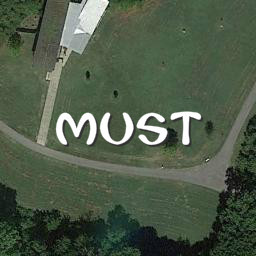
\includegraphics[scale=0.6]{Figs/example.jpg}
	\caption{Example.}
	\label{fig.2.1}
\end{figure}

